% ============================================================
% Kapitel 1: Einführung
% ============================================================
\chapter{Einführung}

Kaum ein anderes Thema hat die Technologiebranche in den letzten Jahren so geprägt wie künstliche Intelligenz.
Um im globalen Wettbewerb um die leistungsfähigsten Sprachmodelle bestehen zu können, investieren
Unternehmen Milliardensummen in Recheninfrastruktur.
Ein eindrückliches Beispiel hierfür ist \textit{Colossus}, der von Elon Musks KI-Firma xAI errichtete GPU-Cluster:
Mit 100\,000 NVIDIA HGX H100 GPUs, verteilt auf vier wassergekühlte Hallen in Memphis, Tennessee, stellt er den bislang größten KI-Supercomputer der Welt dar und dient dem Training des generativen Modells Grok~\cite{brendel2025colossus}.
Die für solche Systeme benötigte Hardware stammt nahezu ausschließlich vom Branchenführer NVIDIA, der über 90\,\% des Marktes für KI-GPUs hält.
CEO Jensen Huang bezifferte das Auftragsvolumen des Unternehmens für die Jahre 2025 und 2026 auf rund 500 Milliarden US-Dollar -- ein Zeichen für die nach wie vor rasant wachsende Nachfrage~\cite{leswing2025nvidia}.
Dieser massive Ausbau von Rechenzentren hat weitreichende energetische Konsequenzen:
Laut einer Prognose der Internationalen Energieagentur (IEA) könnte sich der weltweite Stromverbrauch von Rechenzentren bis 2030 verdoppeln, wobei der Bedarf sogenannter beschleunigter Server -- wie sie für KI-Workloads eingesetzt werden -- im Zeitraum 2025 bis 2030 um 225\,\% steigt~\cite{janson2025rechenzentren}.

Angesichts dieser Entwicklungen stellt sich die Frage, ob der Betrieb solcher ressourcenintensiver Modelle für jeden Anwendungsfall notwendig ist.
Insbesondere in industriellen Einsatzszenarien -- etwa auf Edge-Geräten oder Robotern in der Produktion, die häufig keine dauerhafte Internetverbindung wünschen oder zulassen -- bieten sich deutlich kleinere, spezialisierte Modelle an.
Diese können \textit{On-Premise}, also vor Ort auf eigener Hardware, betrieben werden und erfordern weder die enormen Rechenkapazitäten cloudbasierter Infrastrukturen noch den damit verbundenen Energieverbrauch.
Die vorliegende Arbeit untersucht daher, inwieweit solche lokalen Modelle für spezifische Anwendungsfälle eine praktikable und effiziente Alternative zu den großen, cloudbasierten Sprachmodellen darstellen.



\section{Problemstellung}

Der rasante Ausbau cloudbasierter KI-Dienste wirft neben technischen und energetischen Fragen zunehmend auch Bedenken hinsichtlich \textbf{Datenhoheit}, \textbf{Sicherheit} und \textbf{technologischer Unabhängigkeit} auf.
Die dominierenden KI-Plattformen -- darunter Dienste von OpenAI, Google und Anthropic -- werden überwiegend in Rechenzentren US-amerikanischer Hyperscaler betrieben.
Daten, die an diese Modelle übermittelt werden, verlassen damit häufig den europäischen Rechtsraum und unterliegen potenziell dem Zugriff ausländischer Behörden, etwa im Rahmen des US-amerikanischen CLOUD Act.
Laut dem Bitkom Cloud Report 2025 sehen 78\,\% der deutschen Unternehmen eine zu starke Abhängigkeit von US-Cloud-Anbietern, und für 97\,\% der befragten Cloud-Nutzer spielt die Herkunft des Anbieters bei der Auswahl eine wesentliche Rolle~\cite{bitkom2025cloud}.

Für produzierende Unternehmen verschärft sich diese Problematik zusätzlich:
Sensible Produktionsdaten, Prozessparameter oder Qualitätsinformationen dürfen aus Gründen des Geschäftsgeheimnisschutzes und der Compliance häufig das Unternehmensnetzwerk nicht verlassen.
Roboter und Edge-Geräte in der Fertigung operieren zudem oft in Umgebungen ohne zuverlässige oder gewünschte Internetanbindung.
Die Nutzung cloudbasierter KI-Modelle ist in solchen Szenarien daher entweder nicht möglich oder mit erheblichen Risiken verbunden.
Es stellt sich somit die Frage, ob kleinere, spezialisierte Sprachmodelle, die vollständig vor Ort, also On-Premise, betrieben werden können, eine sichere, unabhängige und zugleich leistungsfähige Alternative für industrielle Anwendungsfälle darstellen. Bevor jedoch auf die Problematik eingegangen wird, wird im folgenden Kapitel der Stand der Technik erläutert.

\section{Stand der Technik}

Wie im vorherigen Kapitel bereits aufgegriffen, beschäftigt sich diese Arbeit primär mit der Verwendung von Large Language Models auf Edge"=Geräten und On"=Premise"=Infrastrukturen.
Der Begriff des maschinellen Lernens ist in der Informatik keineswegs neu -- bereits seit Anfang des 21.\ Jahrhunderts existieren Algorithmen, die nichtlineare Zusammenhänge in Daten erkennen können.
Einen entscheidenden Durchbruch markierte das Jahr 2017, als Vaswani et al.\ die sogenannte Transformer"=Architektur vorstellten.
Diese Architektur ermöglichte den Übergang von sequenzieller zu paralleler Datenverarbeitung und erlaubte es, diese Parallelisierung mit der massiven Rechenleistung moderner GPUs zu koppeln, um deutlich größere Datenmengen effizient zu verarbeiten.

Auf dieser Grundlage entstanden Modelle, die in der Lage sind, komplexe Muster in umfangreichen Textkorpora zu erkennen und natürlichsprachliche Ausgaben zu erzeugen -- sogenannte \textit{Large Language Models} (LLMs).
Laut Kasneci et al.\ (2023) ist ein LLM ein künstliches Intelligenzsystem, das auf einer riesigen Menge von Textdaten trainiert wurde, um natürliche Sprache zu interpretieren und menschenähnliche Antworten auf textbasierte Eingabeaufforderungen oder Fragen zu generieren~\cite{llm_definition}.

Seitdem hat sich die Leistungsfähigkeit dieser Modelle rasant weiterentwickelt, wobei die Parameteranzahl und damit auch der Ressourcenbedarf stetig gestiegen sind.
In Abbildung~\ref{fig:vram_llm} werden die geschätzten Mengen an schnell zugänglichem Grafikspeicher (VRAM) dargestellt, die für den Betrieb aktueller Flagschiffmodelle erforderlich sind.
Für Edge"=Geräte, die auf eine begrenzte Speicherkapazität angewiesen sind, kommen diese Modelle daher nicht in Frage.

\begin{figure}[H]
    \centering
    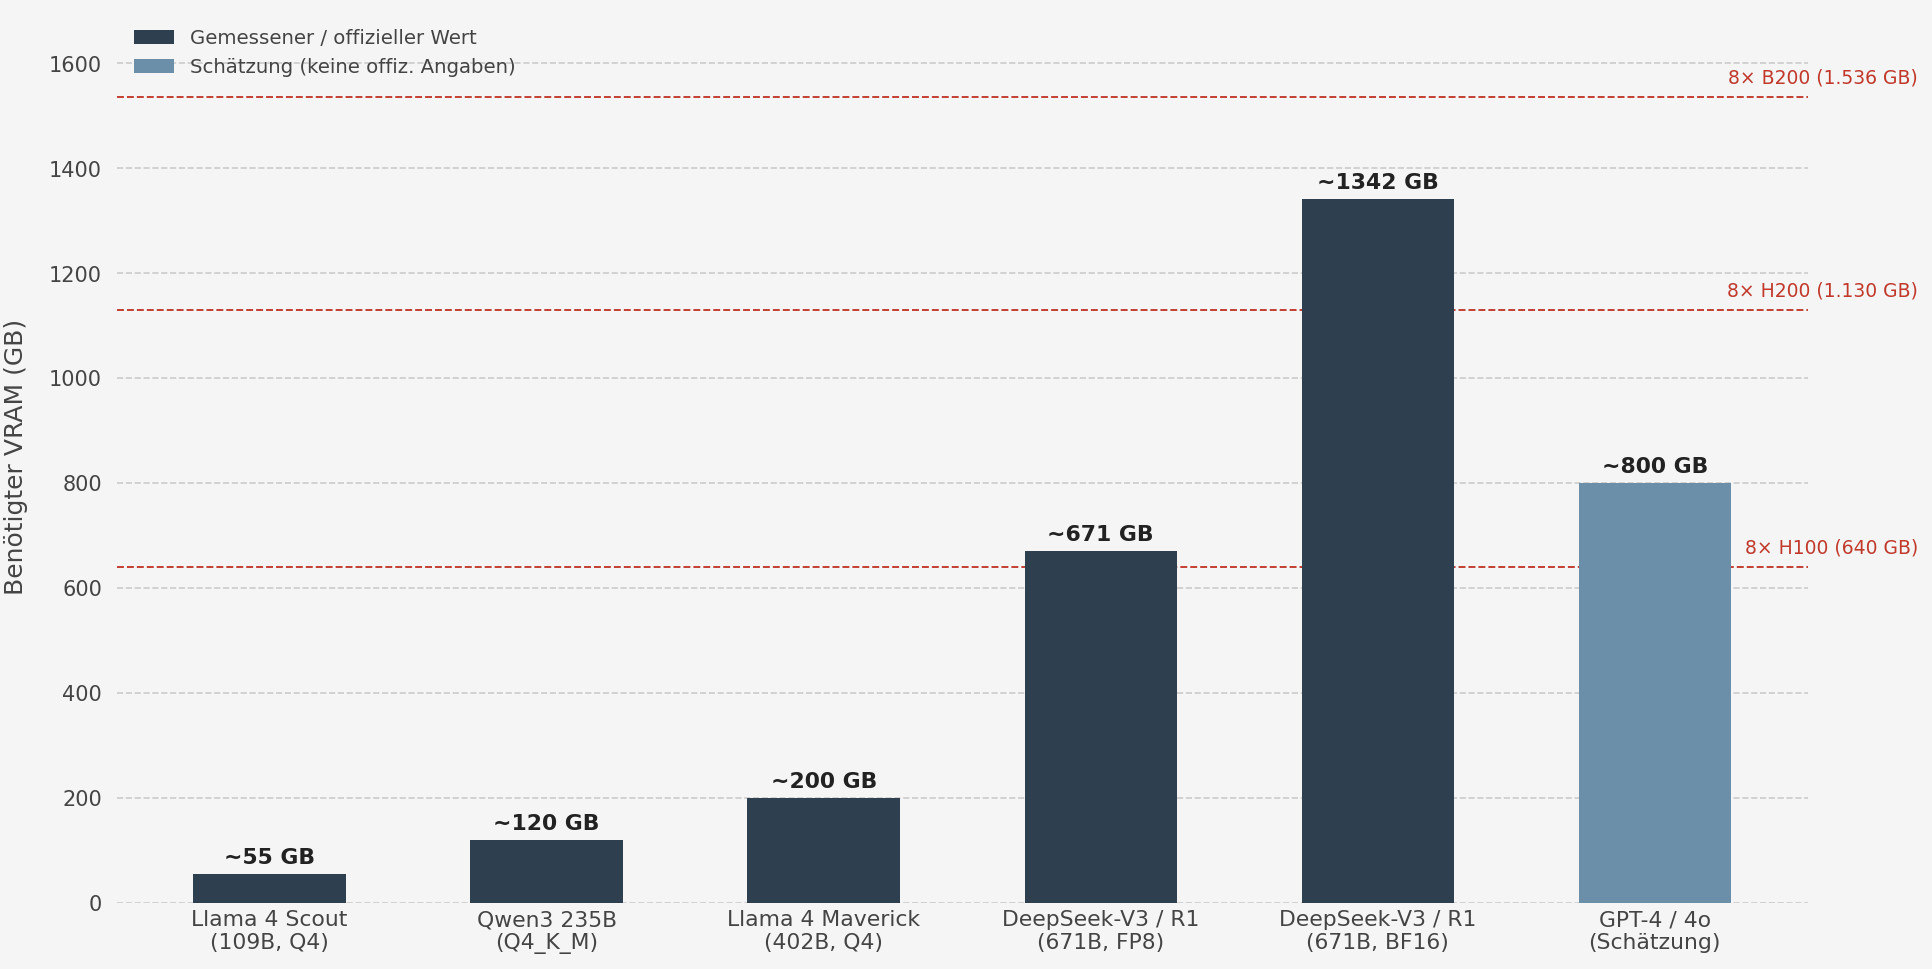
\includegraphics[width=0.83\textwidth]{abbildungen/vramllm.jpg}
    \caption{Geschätzter VRAM-Bedarf aktueller LLM-Flagschiffmodelle}
    \label{fig:vram_llm}
\end{figure}

Die leistungsstärksten quelloffenen Modelle, die für einen On"=Premise"=Betrieb relevant sind, werden in Abbildung~\ref{fig:llm_onpremise} gegenübergestellt.
Dabei wird der Chatbot-Arena-Elo-Score -- ein crowdsource-basiertes Maß für die vom Nutzer wahrgenommene Antwortqualität -- dem jeweiligen VRAM"=Bedarf bei 4"=Bit"=Quantisierung (INT4) gegenübergestellt.
Modelle, die mit maximal 48\,GB VRAM auskommen, lassen sich bereits auf einer einzelnen Consumer"=GPU betreiben und sind somit für Edge- und On"=Premise"=Szenarien besonders interessant.
Prinzipiell sind die jeweils neuesten Modellgenerationen die leistungsstärksten; zum Zeitpunkt der Erstellung dieser Arbeit stellt Qwen~3.5 von Alibaba mit einem Arena-Elo-Score von 1450 das leistungsstärkste quelloffene Modell dar.

\begin{figure}[H]
    \centering
    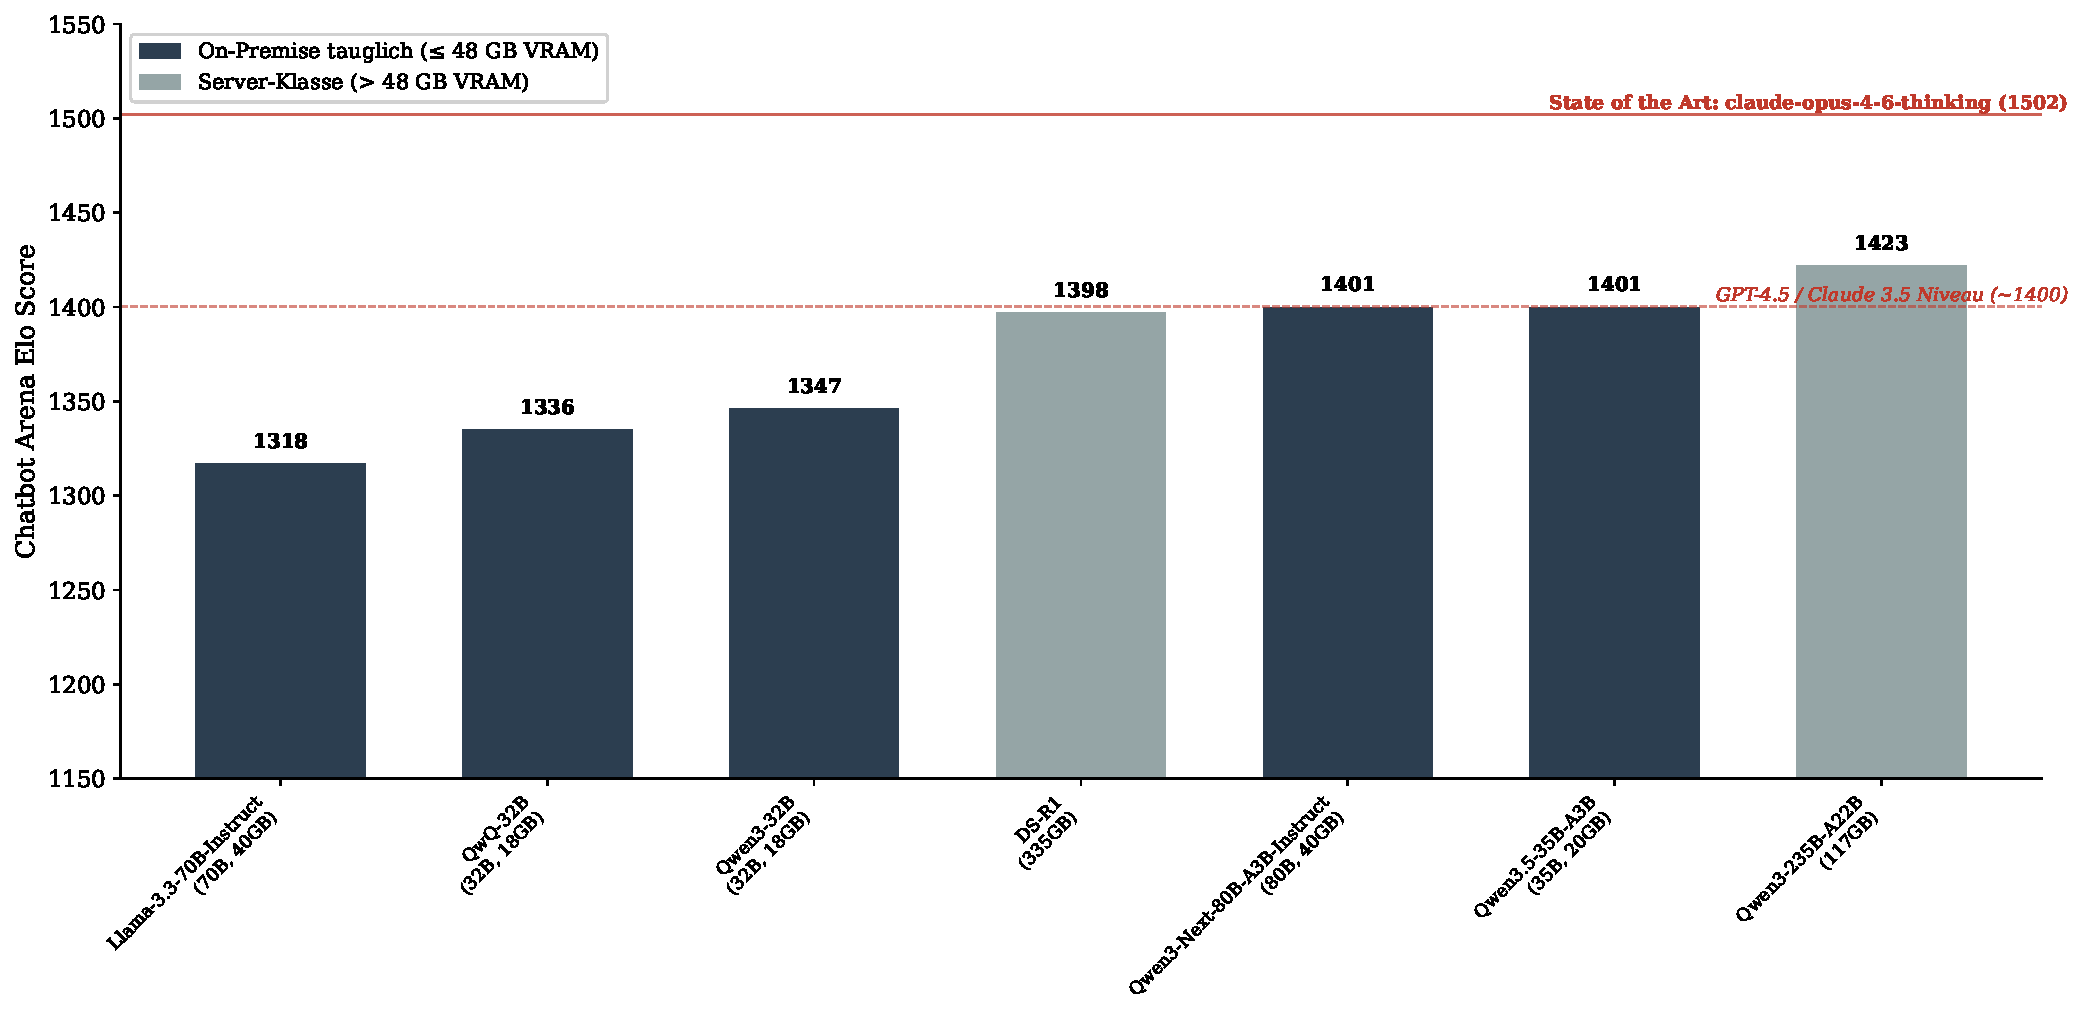
\includegraphics[width=0.95\textwidth]{abbildungen/llm_onpremise_leaderboard.pdf}
    \caption{Vergleich quelloffener LLMs: Chatbot Arena Elo vs.\ VRAM-Bedarf (INT4). Grün hervorgehobene Modelle sind für den Betrieb auf einer einzelnen Consumer-GPU ($\leq$\,48\,GB) geeignet. Datenquelle: onyx.app/self-hosted-llm-leaderboard, Stand März 2026.}
    \label{fig:llm_onpremise}
\end{figure}

\section{Zielsetzung}

Im Rahmen dieser Forschungsarbeit wird der Einsatz von On-Premise-LLMs, also vor Ort betriebenn, am Beispiel der Anwendungsmöglichkeit im Innovationszentrum für Produktion und Logistik (im folgenden IZPL) der OTH Regensburg untersucht. Dabei wird auf öffentlich verfügbare Modelle zurückgegriffen, die lokal auf einem Server des IZPL betrieben werden. Ziel ist es, die Grundlagen, technischen Anforderungen und Möglichkeiten solcher Systeme für künftige robotiknahe Anwendungen zu analysieren. Konkret dient diese wissenschaftliche Arbeit als Fundament für eine Abschlussarbeit im IZPL Regensburg.


\section{Aufbau der Arbeit}

Zunächst erfolgt eine Einführung in die mathematischen Konzepte, auf denen die Modelle basieren. Die im Folgenden aufgeführten Hardwarespezifikationen legen dar, welche Computing-Kapazitäten erforderlich sind, um sogenannte "künstliche Intelligenzen" (KI) zu erschaffen. Nach Evaluation einer Testanwendung in Kapitel 4 werden Sicherheits- und Fehlerbilder aufgezeigt. Die vorliegende Arbeit findet ihren Abschluss in Kapitel 6, das einen Ausblick auf zukünftige Forschungsgebiete gibt und ein Fazit zieht.
